\documentclass[11pt,DIV=9, letterpaper, oneside, openright]{scrartcl}
\usepackage{graphicx}
\usepackage[utf8]{inputenc}
\usepackage[spanish]{babel}
\title{Edición, mantenimiento y evaluación de una aplicación web para mostrar el fenómeno del suicidio}
\subtitle{Reporte de actividades Febrero-2024}
\author{José Adrián Rodríguez González }
\date{Febrero 2024}
\begin{document}

\maketitle

\section{Introducción}
Las tareas a realizar y a redactar en el presente reporte de actividades son:
 \begin{itemize}
     \item Corrección de errores
     \item Pruebas de despliegue en diversas resoluciones de la plataforma
     \item Cambios de los elementos gráficos.
 \end{itemize}
 En base al plan de trabajo se realizó de la siguiente forma:
 \section{Corrección de errores}

 Al realizar las correcciones de errores se encontraron fallas en la visibilidad en distintas resoluciones de pantalla, por ejemplo, frases que se compactaban entre sí, imágenes que se desbordaban de la pantalla, el corte de la cuerda, entre otros. La principal teoría que se tenía era que posiblemente se estaban utilizando medidas absolutas, por lo que al cambiar la resolución, las fuentes e imágenes no podían adaptarse a la \textit{nueva resolución} debido a que se habían encarcelado a las de un tamaño determinado de pantalla. Así que, el primer gran cambio fue en los archivos principales de la aplicación, el archivo \textit{App.jsx} y el archivo \textit{App.css}. Durante el proceso de intercambio de medidas absolutas a relativas, parecía que al eliminar un bug, aparecían más bugs, por lo que se tuvo que encontrar la raíz del problema para que los bugs \textit{nuevos} se fueran eliminado por sí solos. El principal cambio, fue el aumento de páginas del componente Parallax  ajustar las fuentes de texto; para ello, se debió de buscar sus argumentos a su vez de como funcionaba el componente \cite{Parallax-react}.
 Con ello, se pudo reducir la cantidad de errores que producía al cambiar las resoluciones de pantalla. Sin embargo, a pesar de que se intercambiaron las fuentes de los estilos a unos con mayor adaptabilidad en las pantallas, aun se presentaban dos grandes problemas:

 \begin{enumerate}
     \item El corazón no se encontraba en el centro
     \item La cuerda se cortaba y se movía conforme cambiarás la pantalla.
 \end{enumerate}

 Estos problemas y sus soluciones forman parte de las siguientes secciones, debido a que se encontraron al probarlos en las distintas pantallas
 
 \section{Pruebas de despliegue en diversas resoluciones de la plataforma}
 
 Para que un sitio web sea exitoso, debe de ser \emph{responsive}, es decir, que su GUI sea adaptativa a las distintas resoluciones. Mientras se realizaron las primeras soluciones a los problemas encontrados en el sitio, se visualizó un problema, y es que la cuerda a menor tamaño de ancho de la pantalla, se cortaba o desplazaba más, por lo que de la misma forma, se realizo un intercambio de valores absolutos a relativos a su vez, que su propiedad de posición estuviera más enlazada con la forma que presente cada pantalla a que solo permanezca fija con un valor determinado.
 \begin{figure}[h]
 \centering
 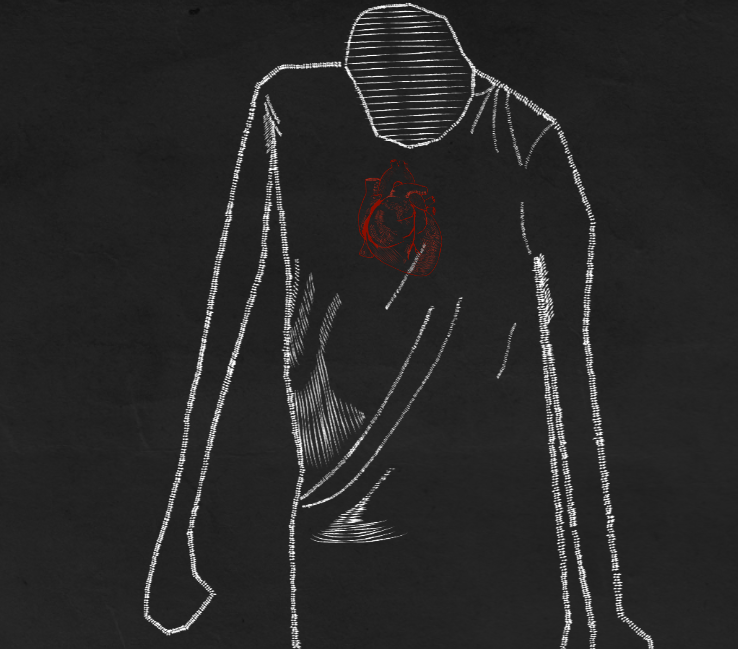
\includegraphics[width=8cm]{body.png}
 \end{figure}

 Con ello se resolvió el problema de que la cuerda se cortaba a su vez de que se añadió una nueva imagen para empatar el final de la cuerda.
 
 \begin{figure}[h]
 \centering
 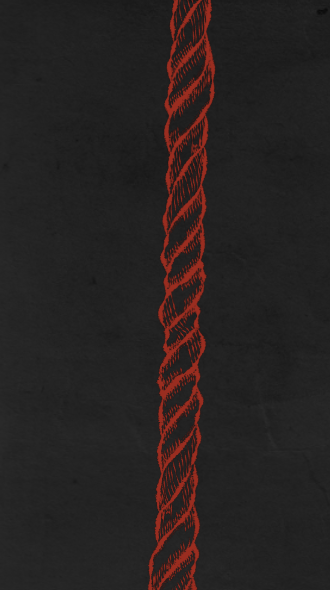
\includegraphics[width=8cm]{image.png}
 \end{figure}
 El problema con el corazón fue ligeramente distinto, sin embargo era significativo, debido a que su posición estaba más enlazada al \emph{body} del documento que la imagen del cuerpo del persona. Así sus propiedades de posición tanto del cuerpo como del corazón cambiaron, haciendo que el cuerpo en primeras instancias sí estuviera afiliado al body del documento y el corazón al cuerpo, haciendo de tal forma que el corazón se pueda centrar al cuerpo y que cambiara de tamaño respecto a la resolución.
 
 \section{Cambios en los elementos gráficos}
 El cambio en los elementos gráficos fueron ligeras modificaciones a las ilustraciones. A su vez que los cambios subsecuentes para que la página pudiera adaptarse mejor a las distintas resoluciones.

 Sin embargo, en el momento de terminar todos los cambios, se encontró un nuevo error y era el como en la página aparecía una  'animación'  que no debía estar ahí. Debido a la complejidad de este error, se decidió no atender en el tiempo que comprende este reporte.  

\bibliographystyle{plain} 
\bibliography{references}
\end{document}
